\documentclass[conference]{IEEEtran}

\usepackage{amsmath, amssymb, amsfonts}
\usepackage{algorithmic}
\usepackage{graphicx}
\usepackage{textcomp}
\usepackage{xcolor}
\usepackage{tikz}
\usepackage[colorlinks = true]{hyperref}
\usepackage[hyperref = true, citestyle = authoryear]{biblatex}

\addbibresource{not-chat-gpt.bib}
\def\BibTeX{{\rm B\kern-.05em{\sc i\kern-.025em b}\kern-.08em
    T\kern-.1667em\lower.7ex\hbox{E}\kern-.125emX}}

\begin{document}

\title{Modeling Musical Expression as a Score-Performance Hidden Markov Model With Invariant Risk Minimization}

\author{\IEEEauthorblockN{Quinn Ouyang}
    \IEEEauthorblockA{\textit{School of Music, College of Fine and Applied Arts} \\
        \textit{University of Illinois Urbana-Champaign}\\
        Champaign, Illinois, United States \\
        \href{mailto:qouyang3@illinois.edu}{qouyang3@illinois.edu}}
}

\maketitle

\begin{abstract}
    We define score-performance analysis as a novel task of comparing a performance/relization of music to its symbolic representation (e.g.\ a recording vs.\ sheet music). One perspective of this task focuses on understanding \textit{how} a musician performs rather than \textit{what} they perform, i.e.\ obtaining a ``profile'' of their musical interpretation, style, etc.\ across their performances. We propose modeling this as a hidden Markov model where we can directly observe scores and performances, but not performance profiles. Applying invariant risk minimization yields on this chain yields an interpretable representation of musical expression that minimizes score information (in theory–we have not proved nor verified this).
\end{abstract}

\begin{IEEEkeywords}
    music score, musical expression, hidden Markov model, invariant risk minimzation, information theory
\end{IEEEkeywords}

\section{Introduction}
While most audio and music computation research centers around fairly well-defined tasks (e.g\ automatic music transcription or instrument classification), developments on more subjective problems remains scarce. One of the biggest gaps in the field is bridging between symbolic music representations and audio, especially as the academic community tends to seperate these domains into music information retrieval and signal processing, respectively. We take on the challenge of modeling the inherently human process of musical performance. \parencite{Cacino-Chacon}

Fundamentally, scores are manuscripts that represent a musical idea. They usually detail a sequence of pitches (notes) with broad performance directions (instruments, tempos, dynamics, etc.) to interpret and realize as a performance. As musicians inevitably read and play music differently, multiple performances of varying acoustic characteristics can come from a single score. Therefore, through a simplified perspective, a score can map to multiple performances but a performance can map to only one score.

We focus on quantifying musical interpretation, i.e.\ the transition between a music score and a performance of it.

\section{Related Work}

\subsection{Quantifying Musical Expression}

Very little computational research surrounding musical interpretation of scores exist. \parencite{Cacino-Chacon, Friberg}

\subsection{Hidden Markov Models}

\subsection{Invariant Risk Minimization}

\section{Formulation}

Our goal is to learn a representation of musical expression \(Y\) from paired score-performance data \(X := \{(s_i, p_i)\}_{i=1}^N\) where \(s_i \in X_s\) and \(p_i \in X_p\).

\subsection{Minimizing Risk Across Environments}

From the perspective of IRM, we inevitably sample scores from different environments, so \(X\) technically consists of sets of score-performance pairs where \(X^e := \{(s_i^e, p_i^e)\}_{i=1}^N, \forall e \in E\) where \(s_i^e \in X_s^e\) and \(p_i^e \in X_p^e\) \parencite{Arjovsky, Huszar}.

To form a somewhat realistic structural equation model, we make several simplifying assumptions in the score-to-performer flow to relate these random variables.
\begin{itemize}
    \item A score \(s_i^e \in X_s^e\) only depends on its environment \(e \in E\), i.e.\ \(p(s_i^e, e) = p(s_i^e \mid e) p(e)\)
    \item A performer's profile \(y \in Y\) only depends on the score \(s_i^e\) it receives, i.e.\ \(p(y_i, s^e) = p(y \mid s_i^e)\)
    \item A performer's performance \(p_i^e \in X_p^e\) depends on its score \(s_i^e\) and profile \(p_i^e\), i.e.\ \(p(p_i^e, s_i^e, y_e) = p(p_i^e \mid s_i^e, y_e) p(s_i^e, y_e)\)
\end{itemize}

The chain rule of conditional probabilities yields: \parencite{Berdahl, Degirmenci}
\begin{align*}
    p(e, s_i, p_i, y)
     & = p(y \mid e, s_i, p_i) p(e, s_i, p_i)                        \\
     & = p(y \mid e, s_i, p_i) p(p_i \mid e, s_i) p(e, s_i)          \\
     & = p(y \mid e, s_i, p_i) p(p_i \mid e, s_i) p(s_i \mid e) p(e) \\
     & = p(y \mid s_i, p_i) p(p_i \mid s_i) p(s_i \mid e) p(e)
\end{align*}

\subsection{As a Communications Channel}

We can interpret a performer's profile as a semi-deterministic encoder from a score \(s_i^e\) to a performance \(p_i^e\) which maximizes the mutual information between the two (though always performing music as closely to what a composer writes is debatable from a musicology standpoint). \parencite{Berdahl, Meyer}

\subsection{As a Hidden Markov Model}

We can model this as a simplified feed-forward HMM\@:
\begin{itemize}
    \item A set of score environments \(E\) directly influences the distribution of observed scores \(X_s\)
    \item A random variable \(Y\) describing a performance profile, dependent on the input score
    \item A set of performances \(X_p\) bijectively mapped their corresponding scores
\end{itemize}

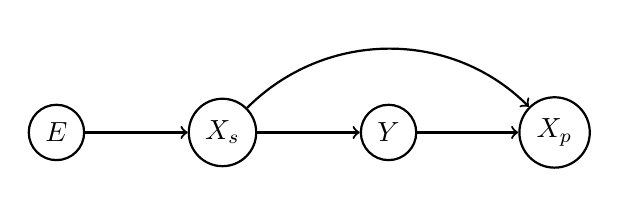
\begin{tikzpicture}[auto, node distance=6em, thick, N node/.style={circle, draw, minimum size=2em}]
    \node[N node] (E) {\(E\)};
    \node[N node] (Xs) [right of=E] {\(X_s\)};
    \node[N node] (Y) [right of=Xs] {\(Y\)};
    \node[N node] (Xp) [right of=Y] {\(X_p\)};

    \path
    (E) edge[->] node {} (Xs)
    (Xs) edge[->] node {} (Y)
    (Y) edge[->] node {} (Xp)
    ;

    \draw[->] (Xs) to[out=45, in=135] (Xp);
\end{tikzpicture}

\nocite{*}
\printbibliography

\end{document}
